\subsection{Theoretische Grundlagen}
\subsubsection{Zeemann-Effekt}
Beim Zeemann-Effekt wird die Aufspaltung der Energieniveaus in Atomen durch Anlegen eines Magnetfeldes beobachtet. In unserem Experiment beobachten wir Übergänge von Elektronen im Cadmium-Atom. Die für uns wichtige Größe ist dabei der Gesamtdrehimpuls, der sich aus Bahndrehimpuls und Spin zusammensetzt, $\vec{J}=\vec{L}+\vec{S}$. Einen Zustand mit Drehimpulsquantenzahl $l$ (notiert als S,P,D,...), Spinquantenzahl $s$ und Gesamtdrehimpulsquantenzahl $j$ schreiben wir mit der spektroskopischen Notation als
\begin{align*}
  ^{2s+1}l_j.
\end{align*}
Das Atom soll sich nun in einem homogenen Magnetfeld $B$ entlang der $z$-Achse befinden (Quantisierungsachse). Dadurch wird die vorherige Entartung der Energieniveaus in der $J_z$ Quantenzahl $m_j$ aufgehoben (siehe Abb. \ref{fig:level}). In Abhängigkeit der alten Energie $E_0$ ist die neue Energie dann\cite{shankar}
\begin{align*}
  E=E_0-\frac{\mu_\mathrm{B}}{\hbar}\left( m_j+m_s\right),
\end{align*}
wobei $m_s$ die Quantenzahl zum Spin in $z$-Richtung, $\mu_\mathrm{B}$ das Bohrsche Magneton und $\hbar$ das Plancksche Wirkungsquantum ist.

\begin{figure}[h]
  \centering
  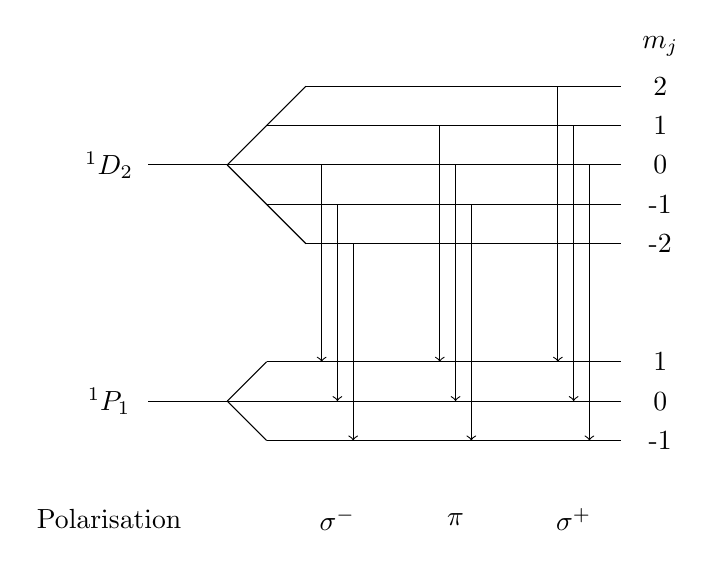
\begin{tikzpicture}
    \draw (0,0)--(6,0);
    \draw (1,0)--(2,1);
    \draw (1,0)--(2,-1);
    \draw (1.5,0.5)--(6,0.5);
    \draw (2,1)--(6,1);
    \draw (1.5,-0.5)--(6,-0.5);
    \draw (2,-1)--(6,-1);
    \draw (-0.5,0) node {$^1D_2$};
    \draw (6.5,1.5) node {$m_j$};
    \draw (6.5,1) node {2};
    \draw (6.5,0.5) node {1};
    \draw (6.5,0) node {0};
    \draw (6.5,-0.5) node {-1};
    \draw (6.5,-1) node {-2};

    \draw (0,-3)--(6,-3);
    \draw (1,-3)--(1.5,-2.5);
    \draw (1,-3)--(1.5,-3.5);
    \draw (1.5,-2.5)--(6,-2.5);
    \draw (1.5,-3.5)--(6,-3.5);
    \draw (-0.5,-3) node {$^1P_1$};
    \draw (6.5,-2.5) node {1};
    \draw (6.5,-3) node {0};
    \draw (6.5,-3.5) node {-1};

    \draw[->] (2.2,0)--(2.2,-2.5);
    \draw[->] (2.4,-0.5)--(2.4,-3);
    \draw[->] (2.6,-1)--(2.6,-3.5);

    \draw[->] (3.7,0.5)--(3.7,-2.5);
    \draw[->] (3.9,0)--(3.9,-3);
    \draw[->] (4.1,-0.5)--(4.1,-3.5);

    \draw[->] (5.2,1)--(5.2,-2.5);
    \draw[->] (5.4,0.5)--(5.4,-3);
    \draw[->] (5.6,0)--(5.6,-3.5);
    
    \draw (-0.5,-4.5) node {Polarisation};
    \draw (2.4,-4.5) node {$\sigma^-$};
    \draw (3.9,-4.5) node {$\pi$};
    \draw (5.4,-4.5) node {$\sigma^+$};
  \end{tikzpicture}
  \caption{Ausgewählte Übergänge in Cadmium}
  \label{fig:level}
\end{figure}  

In diesem Experiment werden elektrische Übergänge 
\begin{align*}
^1D_2 \ \rightarrow  \ ^1P_1 
\end{align*}
untersucht, es gilt also $m_s=0$. Dies entspricht dem Übergang eines Valenzelektrons. Die Übergänge können durch die Änderung der Quantenzahl $m_j$ für den Gesamtdrehimpuls entlang der Quantisierungsachse charaktersiert werden. In erster Ordnung sind nur Übergänge mit $\Delta m_j=0, \ 1, \ -1$ erlaubt. Die Polarisation des ausgesandten Lichtes ist dabei jeweils $\pi$, $\sigma ^+$ und $\sigma^-$.

Bei den betrachteten Übergängen ändert sich die Energie des $\pi$-polarisierten Lichtes also nicht mit dem Magnetfeld (wegen $m_s=0$). Bei dem $\sigma^{\pm}$ Übergängen ändert sich die Energie der Photonen mit dem Magnetfeld um
\begin{align}
  \delta E=\mp \mu_B B.
  \label{eq:de}
\end{align}
Wichtig für die Beobachtung ist, dass das Licht mit $\pi$-Polarisation nicht parallel zum Magnetfeld ausgesandt wird, während das zirkular polarisierte Licht hauptsächlich in Richtung des Magnetfeldes ausgesandt wird.
\subsubsection{Fabry-Pérot-Etalon}
Um die Energieverschiebung aus Gleichung $\ref{eq:de}$ zu messen wird ein Fabry-Pérot-Etalon verwendet. Dieses ist ein optischer Resonator bestehend aus einer planparallelen, verspiegelten Glasplatte mit Brechungsindex $n$. Der Strahlengang eines schräg auf den Resonator treffenden Strahles ist in Abbildung \ref{fig:fabry} zu sehen. Anhand der Abbildung lässt sich der Gangunterschied zweier benachbarter Teilstrahlen ermitteln. Somit folgt, dass bei einem Interferenzmaximum von Licht der Wellenlänge $\lambda$
\begin{align}
  2d\sqrt{n^2-\sin^2(\alpha)}=k\lambda
\end{align}
mit $k \in \mathbb{Z}$ gilt. Bei einer Reflektivität $r$ einer einzelnen Oberfläche des Etalons ist das Auflösungsvermögen gegeben durch \cite{fabryperotaufloes}
\begin{align}
  A = \frac{\lambda}{\Delta \lambda}=\frac{2 n d \pi r}{(1-r^2)\lambda}.
\end{align}
Ferner ist die Finesse, definiert durch das Verhältnis aus freiem Spektralbereich $\Delta \lambda$ und Halbwertsbreite $\delta \lambda$, gegeben durch \cite{fabryperotaufloes}
\begin{align}
  F=\frac{\Delta \lambda}{\delta \lambda}=\frac{\pi r}{1-r^2}.
\end{align} 


\begin{figure}[h]
  \centering
  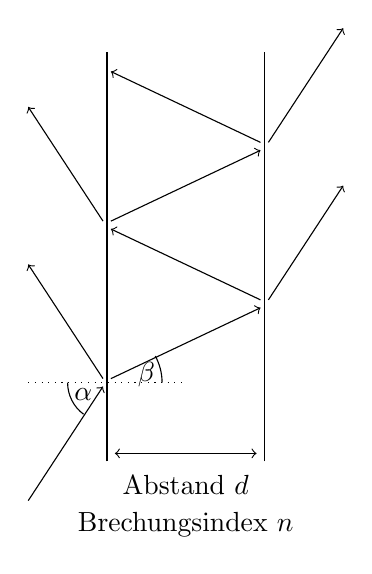
\begin{tikzpicture}
    \draw [<->] (0.1,0.1)--(1.9,0.1);
    \draw (1,-0.3) node {Abstand $d$};
    \draw (1,-0.8) node {Brechungsindex $n$};
    \draw (0,0)--(0,5.2);
    \draw (2,0)--(2,5.2);
    \draw [->] (-1,-0.5)--(-0.05,0.95);
    \draw [->] (-0.05,1.05)--(-1,2.5);
    \draw (-0.5,1) arc (180:233.5:0.5);
    \draw (-0.3,0.85) node {$\alpha$};
    \draw [dotted] (-1,1)--(1,1);
    \draw [->] (0.05,1.05)--(1.95,1.95);
    \draw (0.7,1) arc (0:28.8:0.7);
    \draw (0.5,1.1) node {$\beta$};
    \draw [->] (1.95,2.05)--(0.05,2.95);
    \draw [->] (0.05,3.05)--(1.95,3.95);
    \draw [->] (1.95,4.05)--(0.05,4.95);
    \draw [->] (-0.05,3.05)--(-1,4.5);
    \draw [->] (2.05,2.05)--(3,3.5);
    \draw [->] (2.05,4.05)--(3,5.5);
  \end{tikzpicture}
  \caption{Strahlengang im Fabry-Pérot-Etalon}
  \label{fig:fabry}
\end{figure}

\subsubsection{Dopplerverbreiterung}
Durch die thermische Bewegung der Atome kommt es zur Dopplerverschiebung der Wellenlänge des emittierten Lichtes. Bewegt sich das Atom mit der Geschwindigkeit $v$ auf den Empfänger zu und emittiert ein Photon der Wellenlänge $\lambda$, so misst dieser die Wellenlänge 
\begin{align*}
  \lambda'=\lambda \cdot \left(  1+ \frac{v}{c} \right),
\end{align*} 
wobei $c$ die Lichtgeschwindigkeit ist. Nimmt man an, dass es sich bei dem Gas um ein ideales Gas handelt, gilt für die Geschwindigkeit $v$ jedes Atoms (mit Masse $m$ und Boltzmann-Konstante $k_\mathrm{B}$)
\begin{align*}
  \frac{1}{2} m\ind{K} v^2=\frac{3}{2} k_\mathrm{B} T.
\end{align*}
Durch die Dopplerverschiebung schwankt die Wellenlänge also im Bereich
\begin{align}
  \sigma[\lambda]\ind{Doppler}=\frac{\lambda}{c}\sqrt{\frac{3k\ind{B}T}{m\ind{K}}}.
  \label{equ:doppler}
\end{align}
